\documentclass[t]{beamer}
\usetheme{Warsaw}
\usecolortheme{seahorse}
\usepackage{array}
\usepackage{graphicx}
\usepackage{amssymb,amsmath,mathrsfs,amsfonts}
%\usepackage[colorhighlight,display]{texpower}
%\usepackage{caption}
%\usepackage[all]{xy}
\usepackage{beamerthemesplit}
\mode<presentation>
%\usepackage{pause}
\usepackage{ulem}  % for strikethroughs
\usepackage{cancel} % for strikethroughs in math mode 
\usepackage{tikz}
\usepackage{calc}
\usetikzlibrary{shapes}
\usepackage{hyperref}
\hypersetup{pdfpagemode=FullScreen}
\usepackage{ifthen}
\usepackage{animate}
\usepackage{color}
\usepackage{type1cm}  % used for watermarking
\usepackage{eso-pic}  % used for watermarking
\usepackage[absolute,overlay]{textpos}
  \setlength{\TPHorizModule}{1mm}
  \setlength{\TPVertModule}{1mm}


\theoremstyle{plain}
\newtheorem{prop}{Proposition}
\newtheorem{thm}[prop]{Theorem}
\newtheorem{lem}[prop]{Lemma}
\newtheorem{cor}[prop]{Corollary}
\theoremstyle{definition}
\newtheorem{dfn}{Definition}
\newtheorem{rem}[prop]{Remark}
\newtheorem{ex}{Example}[section]
%\newtheorem{note}{Note}[section]
\newtheorem{exercise}{Exercise}[section]
\newcommand{\nin}{\noindent}
\newcommand{\ds}{\displaystyle}
\renewcommand{\figurename}{Figure \arabic{figure}}
\renewcommand*\familydefault{\sfdefault} 


%%%%%%%%%%%%%%%%%%%%%%%%%%5
%%%%%%%%%%%%%%%%%%%%%%%%%%%%
%%%% some commands that have different meaning in the article/presentation modes

\newcommand{\vvfill}{\mode<presentation>{\vfill}  \mode<article>{\medskip}}   %vfill in presentation only
\newcommand{\sketchspace}{ 
\mode<article>{ \medskip\noindent{\textbf{Sketch:}} \vspace*{6cm} }
\mode<presentation>{ } 
}
\newcommand{\examplespace}{ 
\mode<article>{ \medskip\noindent{\textbf{Example:}} \vspace{6cm} }
\mode<presentation>{ } 
}
\newcommand{\artsmspace}{\mode<article>{\vspace*{2cm}} }  %small space in article mode
\newcommand{\artlargespace}{\mode<article>{\vspace*{6cm}} }  %large space in article mode

\newcommand{\dx}{\,dx}

\newcommand{\soln}{{\textbf{Solution: }}\,\,\,}
\newcommand{\disp}{\displaystyle}

\newcommand{\makedate}{\vvfill
\begin{picture}(10,10)  
\put(260,-20){\mbox{\tiny{\today}}}
\end{picture}
}

\newcommand{\pd}[2]{\dfrac{\partial#1}{\partial#2}}
\newcommand{\pD}[2]{\dfrac{\partial^2#1}{\partial#2^2}}
\newcommand{\pdd}[3]{\dfrac{\partial^2#1}{\partial#2 \partial#3}}


\normalem %stops the ulem package making all the emphs into underlines...
 
 
 
 \newcommand{\refandrev}[2]{
 \begin{small}
  \hspace{6cm}
  \begin{minipage}[r]{8cm}
  Stewart,    Chapter #1   \\
  Review:  \parbox[t]{6cm}{#2}
\end{minipage}
\end{small}
}



\newcounter{heading}
\setcounter{section}{1}
\setcounter{heading}{0}

\newcommand{\makeheading}[1]{\medskip\begin{large}\noindent\textbf{{#1}}\end{large}\smallskip}

%\newenvironment{head}[1]{\medskip\stepcounter{heading}\noindent\textbf{\hspace{0.2cm}{#1}.}}{}
\newcommand{\newhead}[1]{\medskip\stepcounter{heading}\noindent\textbf{\hspace{0.2cm}{#1}.}}


\newcommand{\pf}[1]{\noindent\textit{Proof.}\vspace*{#1 cm}}
\newcommand{\sol}[1]{\noindent\textit{Solution.}\vspace*{#1 cm}}
\newcommand{\further}[1]{\begin{small}\noindent\textit{Further reading: #1}\end{small}}
\newcommand{\exr}[1]{\begin{footnotesize}\noindent\textit{\textbf{Exercises:} Stewart #1}\end{footnotesize}}


% Sets of numbers
\newcommand{\C}{\mathbb{C}}
\newcommand{\RR}{\mathbb{R}}
\newcommand{\Z}{\mathbb{Z}}
\newcommand{\N}{\mathbb{N}}
\newcommand{\Q}{\mathbb{Q}}

% Partitions
\newcommand{\PP}{\mathcal{P}}

% Limits
\newcommand{\limm}[1]{\displaystyle \lim_{x\to #1}}

% Backslash
\newcommand{\bs}{\backslash}

% functions
\newcommand{\cosec}{\mathrm{cosec}}
\newcommand{\cosech}{\mathrm{cosech}}
\newcommand{\sech}{\mathrm{sech}}
\newcommand{\Li}{\mathrm{Li}}
\newcommand{\si}{\mathrm{Si}}
\newcommand{\erf}{\mathrm{erf}}

% Domain and Range
\newcommand{\Dom}{\mathrm{Dom}}
\newcommand{\Codom}{\mathrm{Codom}}
\newcommand{\Range}{\mathrm{Ran}}



\title{Week 12: Sequence}

\begin{document}

\frame{\titlepage}

\setcounter{tocdepth}{2}
\frame{\tableofcontents

}

\AtBeginSection[]
{
\begin{frame}<beamer> 
\tableofcontents[currentsection]  % show TOC and highlight current section
\end{frame}
}

\section{Sequence}

\begin{frame}
\frametitle{Sequence}

\begin{itemize}
	\item \textbf{Definition}: A \textbf{sequence} is an ordered list of numbers
	\item A sequence is often denoted as $\{a_1, a_2, a_3, \cdots, a_n\}$ or $\{a_n\}_{n=1}^{\infty}$ or simply $\{a_n\}$
	\item \textbf{Example}: write out the first three terms of $\left\{\frac{3n + 1}{(n+2)!}\right\}_{n=1}^{\infty}$
\end{itemize}

\begin{align*}
a_1 &= \frac{3 \cdot 1 + 1}{(1+2)!} = \frac{4}{3!} = \frac{4}{3\cdot 2 \cdot 1} = \frac{2}{3}\\
a_2 &= \frac{3 \cdot 2 + 1}{(2+2)!} = \frac{7}{4!} = \frac{7}{4 \cdot 3\cdot 2 \cdot 1} = \frac{7}{24}\\
a_3 &= \frac{10}{5!} = \frac{1}{12}\\
\end{align*}

\end{frame}

\begin{frame}
\frametitle{Arithmetic sequence}

\begin{itemize}
	\item \textbf{Definition}: An \textbf{arithmetic sequence} is a sequence for which consecutive terms have the same common differences.   If $a$ is the first term and $d$ is the common difference,  then the arithmetic sequence has the form:
	$$\{d \cdot k + a\}_{k=0}^{\infty}$$
	\item \textbf{Example}: Write a formula for the general term $a_n$, starting with $n = 0$, of $\{7, 10, 13, 16, 19, \cdots\}$
	\begin{itemize}
		\item Ans: $\{3n + 7\}_{n=0}^{\infty}$	
	\end{itemize}		
\end{itemize}

\end{frame}

\begin{frame}
\frametitle{Geometric sequence}
\begin{itemize}
	\item \textbf{Definition}: A \textbf{geometric} sequence is a sequence for which consecutive terms have the same common ratio.  If $a$ is the first term and $r$ is the common ratio, then a geometric sequence has the form:
	$$\{a \cdot r^{n}\}_{n=0}^{\infty}$$
	\item \textbf{Example}:  Write a formula for  for the general term $a_n$ (start with $n=0$) of $\{3, 0.3, 0.03, 0.003, 0.003, \cdots\}$
	\begin{itemize}
		\item Ans: $\{3 \cdot (0.1)^n\}_{n=0}^{\infty}$
	\end{itemize}
\end{itemize}

\end{frame}

\begin{frame}
\frametitle{Exercise}

For each sequence, write a formula for the general term $a_n$ (start with $n=0$)

\begin{itemize}
	\item $\{\frac{15}{2}, \frac{75}{4}, \frac{375}{8}, \frac{1875}{16}, \cdots\}$
	\item $\{3, -2, \frac{4}{3}, -\frac{8}{9}, \cdots\}$
\end{itemize}

For each sequence, write a formula for the general term $a_n$ (start with $n=1$)

\begin{itemize}
	\item $\{-\frac{2}{9}, \frac{4}{16}, -\frac{8}{25}, \frac{16}{36}, \cdots\}$
	\item $\{-6, 5, -1, 4, 3, 7, 10, 17, \cdots\}$
\end{itemize}

\end{frame}

\begin{frame}
\frametitle{Exercise}

For each sequence, write a formula for the general term $a_n$ (start with $n=0$)

\begin{itemize}
	\item $\{\frac{15}{2}, \frac{75}{4}, \frac{375}{8}, \frac{1875}{16}, \cdots\}$
	\begin{itemize}
		\item Ans: $\left\{\frac{15}{2} \cdot (\frac{5}{2})^n\right\}_{n=0}^{\infty}$
	\end{itemize}
	\item $\{3, -2, \frac{4}{3}, -\frac{8}{9}, \cdots\}$
	\begin{itemize}
		\item Ans: $\left\{3\cdot (-\frac{2}{3})^n\right\}_{n=0}^{\infty}$
	\end{itemize}
\end{itemize}

For each sequence, write a formula for the general term $a_n$ (start with $n=1$)

\begin{itemize}
	\item $\{-\frac{2}{9}, \frac{4}{16}, -\frac{8}{25}, \frac{16}{36}, \cdots\}$
	\begin{itemize}
		\item Ans: $\left\{(-1)^n \frac{2n}{(n + 2)^2}\right\}_{n=1}^{\infty}$
	\end{itemize}
	\item $\{-6, 5, -1, 4, 3, 7, 10, 17, \cdots\}$
	\begin{itemize}
		\item Ans: $a_n = a_{n-1} + a_{n-2}$
	\end{itemize}
\end{itemize}

\end{frame}

\section{Convergence}

\begin{frame}
\frametitle{Convergence}

\begin{itemize}
	\item A sequence $\{a_n\}$ converges if $\displaystyle\lim_{n \to \infty} a_n$ exists as a finite number
	\item That is $\displaystyle\lim_{n \to \infty} a_n = L$ converges if $L$ is ot DNE, $-\infty$ or $\infty$
\end{itemize}

 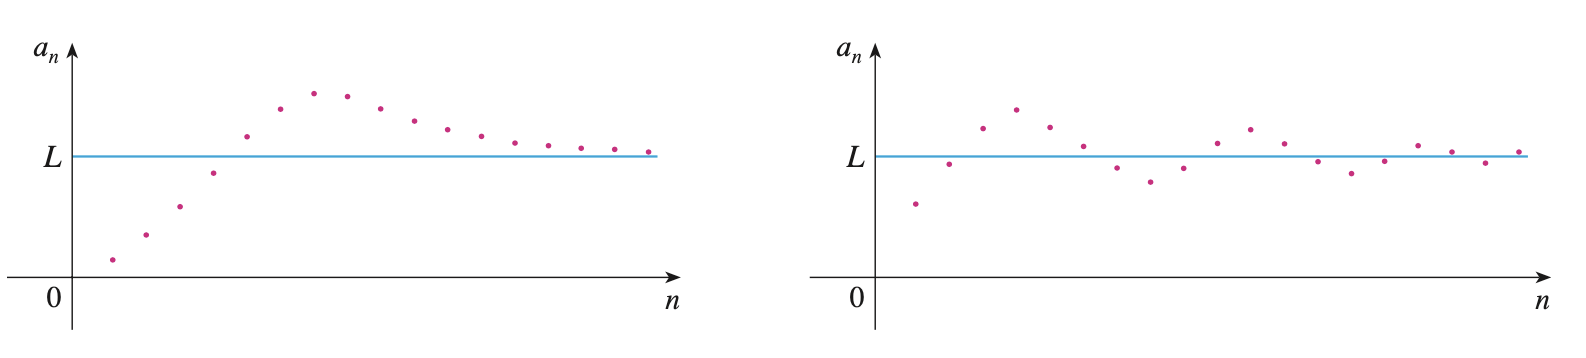
\includegraphics[scale=0.35]{fig/convergence}
 
 \begin{itemize}
	\item We can also say that $\{a_n\}$ converges if $L$ is trapped within certain error bound $\epsilon$ if $N$ is big enough.
\end{itemize}

 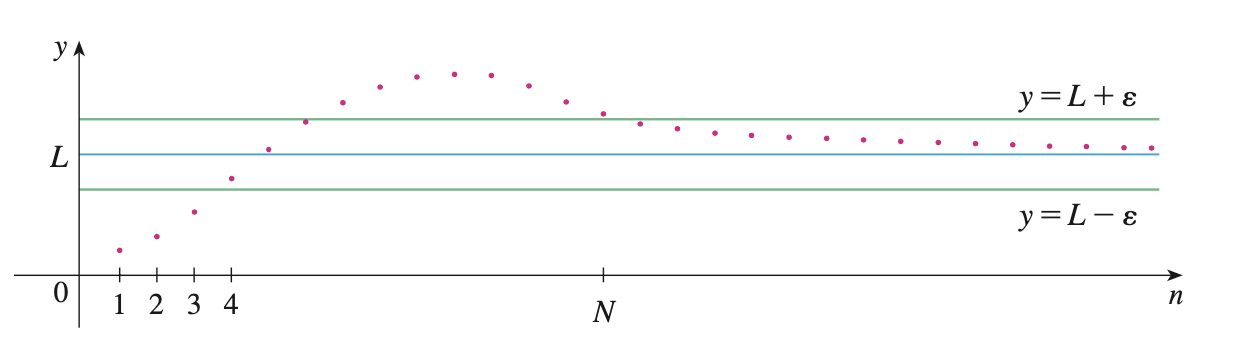
\includegraphics[scale=0.35]{fig/convergence2}

\end{frame}

\begin{frame}

\frametitle{Convergence}

\newhead{Examples}

\begin{itemize}
	\item Converges
	\begin{itemize}
		\item $\left\{\frac{1}{n}\right\}_n^\infty$ since $\displaystyle\lim_{n \to \infty}  \frac{1}{n} = 0$
	\end{itemize}
	\item Diverges
	\begin{itemize}
		\item $\left\{ 2^n \right\}_{n=1}^{\infty}$ since $\displaystyle\lim_{n \to \infty}  2^n = \infty$
	\end{itemize}
	\item Bounded bu still diverges
	\begin{itemize}
		\item $\left\{ (-1)^{n}\right\}_{n=1}^{\infty}$ since it alternates between -1 and 1
	\end{itemize}
\end{itemize}

\end{frame}

\begin{frame}

\frametitle{Example}

\footnotesize

Does $\{a_n\} = \left\{ \frac{\ln(1 + 2e^n)}{n} \right\}_{n=1}^{\infty}$ converges? \pause

\medskip

Suppose $a_n = f(n)$ for some function $f$, where $n = 1, 2, 3, \cdots$.  If $\limm{\infty} f(x) = L$, then $\displaystyle\lim_{n \to \infty}  a_n = L$.

\medskip

We can first look at the sequence as a function and use L'Hospital's Rule or other tricks we learn before to show that the limit exists.

\begin{align*}
\limm{\infty} f(x) &= \limm{\infty} \frac{\ln(1 + 2e^x)}{x} = \frac{\infty}{\infty} && \text{indeterminate form, use L'Hospital Rule}\\
&= \limm{\infty} \frac{\frac{1}{1 + 2e^x} \cdot 2e^x}{1} = \frac{\infty}{\infty} && \text{indeterminate form, use L'Hospital Rule} again\\
&=  \limm{\infty} \frac{2e^x}{2e^x} = 1
\end{align*}

Thus this sequence converges to 1.

\end{frame}

\begin{frame}

\frametitle{Example}

Does $\{ a_n  \} = \left\{  \frac{\cos{n} + \sin{n}}{n^{\frac{2}{3}}}\right\}$ converges? \pause

\medskip

Here we can use the Squeeze Theorem.

\begin{itemize}
	\item We know $-2 \leq \cos(n) + \sin(n) \leq 2$, hence
	\item $\frac{-2}{n^{\frac{2}{3}}} \leq \frac{\cos(n) + \sin(n)}{n^{\frac{2}{3}}} \leq \frac{-2}{n^{\frac{2}{3}}}$, hence
	\item Since $\displaystyle\lim_{n \to \infty}  \frac{-2}{n^{\frac{2}{3}}}  =\displaystyle\lim_{n \to \infty}    \frac{-2}{n^{\frac{2}{3}}}  = 0$, thus $\displaystyle\lim_{n \to \infty}  \frac{\cos(n) + \sin(n)}{n^{\frac{2}{3}}} = 0$
\end{itemize}

\end{frame}

\begin{frame}

\frametitle{Example}

Does $\{0.1, 0.12, 0.123, 0.1234, \cdots, 0.12345\}$ converges? \pause

\medskip

If $\{a_n\}$ is bounded (not smaller or larger than some values) and monotonic (either increasing or decreasing), then it converges.

\medskip

But what number it converges can be mysterious.  (Actually, it is \textit{champernowne} constant.)

\end{frame}

\begin{frame}

\frametitle{Example}

Does $\{r^n\}$ converges? \pause

\begin{itemize}
	\item If $r > 1$, it diverges to $\infty$
	\item If $r = 1$, it converges to 1
	\item If $0 \leq r < 1$, it converges to 0
	\item If $-1 < r < 0$,  it converges to 0
	\item If $r = -1$, it alternates between -1 and 1, thus it diverges
	\item If $r < -1$, it diverges in two direction, thus DNE
\end{itemize}

If we multiply $a$ with the limit, this is also true.

\begin{itemize}
	\item $\{ar^n\}$ converges to 0 when $-1 < r < 1$
	\item $\{ar^n\}$ converges to a when $r = 1$
	\item $\{ar^n\}$ diverges when $r < -1$ or $r > 1$
\end{itemize}

\end{frame}


\begin{frame}

\frametitle{Example}

Does $\left\{  \frac{(-1)^{t} e^{t - 1}}{3^{t + 2}}  \right\}_{t=3}^{\infty}$ converges? \pause

\medskip

\begin{itemize}
	\item Let's simplify to $\frac{(-1)^t e^t e^{-1}}{3^t 3^2} = (\frac{-e}{3})^t \cdot \frac{1}{3^2 e}$
	\item Here we can see that $a = \frac{1}{3^2 e}$ and $r = \frac{-e}{3}$
	\item Here $-1 < r <0$, thus it converges to 0
\end{itemize}

\end{frame}


\begin{frame}

\frametitle{Example}

Does $\left\{   \frac{x-5}{x^2} - \frac{3 \cdot 4^x}{5^x}  \right\}_{x=1}^{\infty}$ converge?

\begin{align*}
&= \limm{\infty} \frac{x - 5}{x^2} - \limm{\infty} \frac{3 \cdot 4^x}{5^x} && \text{r in second term is } \frac{4}{5}\\
&= 0 - 0 = 0 && \text{using limit law}
\end{align*}

Thus it converges to 0.

\end{frame}


\begin{frame}

\frametitle{Exercise}

Is these sequences convergent or divergent?

\begin{itemize}
	\item $\frac{n}{\sqrt{10 + n}}$  %stewart 11.1 Example 5
	\begin{itemize}
		\item Diverges to $\infty$
	\end{itemize}
	\item $\frac{\ln {n}}{n}$
	\begin{itemize}
		\item Converges to 0 using L'Hospital Rule %stewart 11.1 Example 6
	\end{itemize}
	\item $\frac{3 + 5n^2}{n + n^2}$ %stewart 11.1 No. 23
	\begin{itemize}
		\item Converges to 5
	\end{itemize}
	\item $\frac{4^n}{1 + 9^n}$  %stewart 11.1 No. 30
	\begin{itemize}
		\item Converges to 0
	\end{itemize}
\end{itemize}

\end{frame}



\end{document}